
\section {Online Monitoring}

The SVT will be monitored online using the Java based HPS Monitoring Application.
The most basic set of plots can be brough up by issuing the following commands 
from a terminal:  

\begin {itemize}
    \item Log into \textbf{clonpc19} in the counting house as \texttt{hpsrun}
    \item Open a terminal and navigate to \texttt{/home/hpsrun/svt\_monitoring}
    \item Issue the command \texttt{python run\_svt\_monitoring.py} to open the monitoring app
\end {itemize}
Pressing the connect button will bring up plots SVT occupancies, raw hit counts
and raw hit ADC sample amplitudes.  Once a run had ended, the plots need to be 
brough down manually.

\subsection {Occupancies}

\begin{figure}[h!]
    \centering
    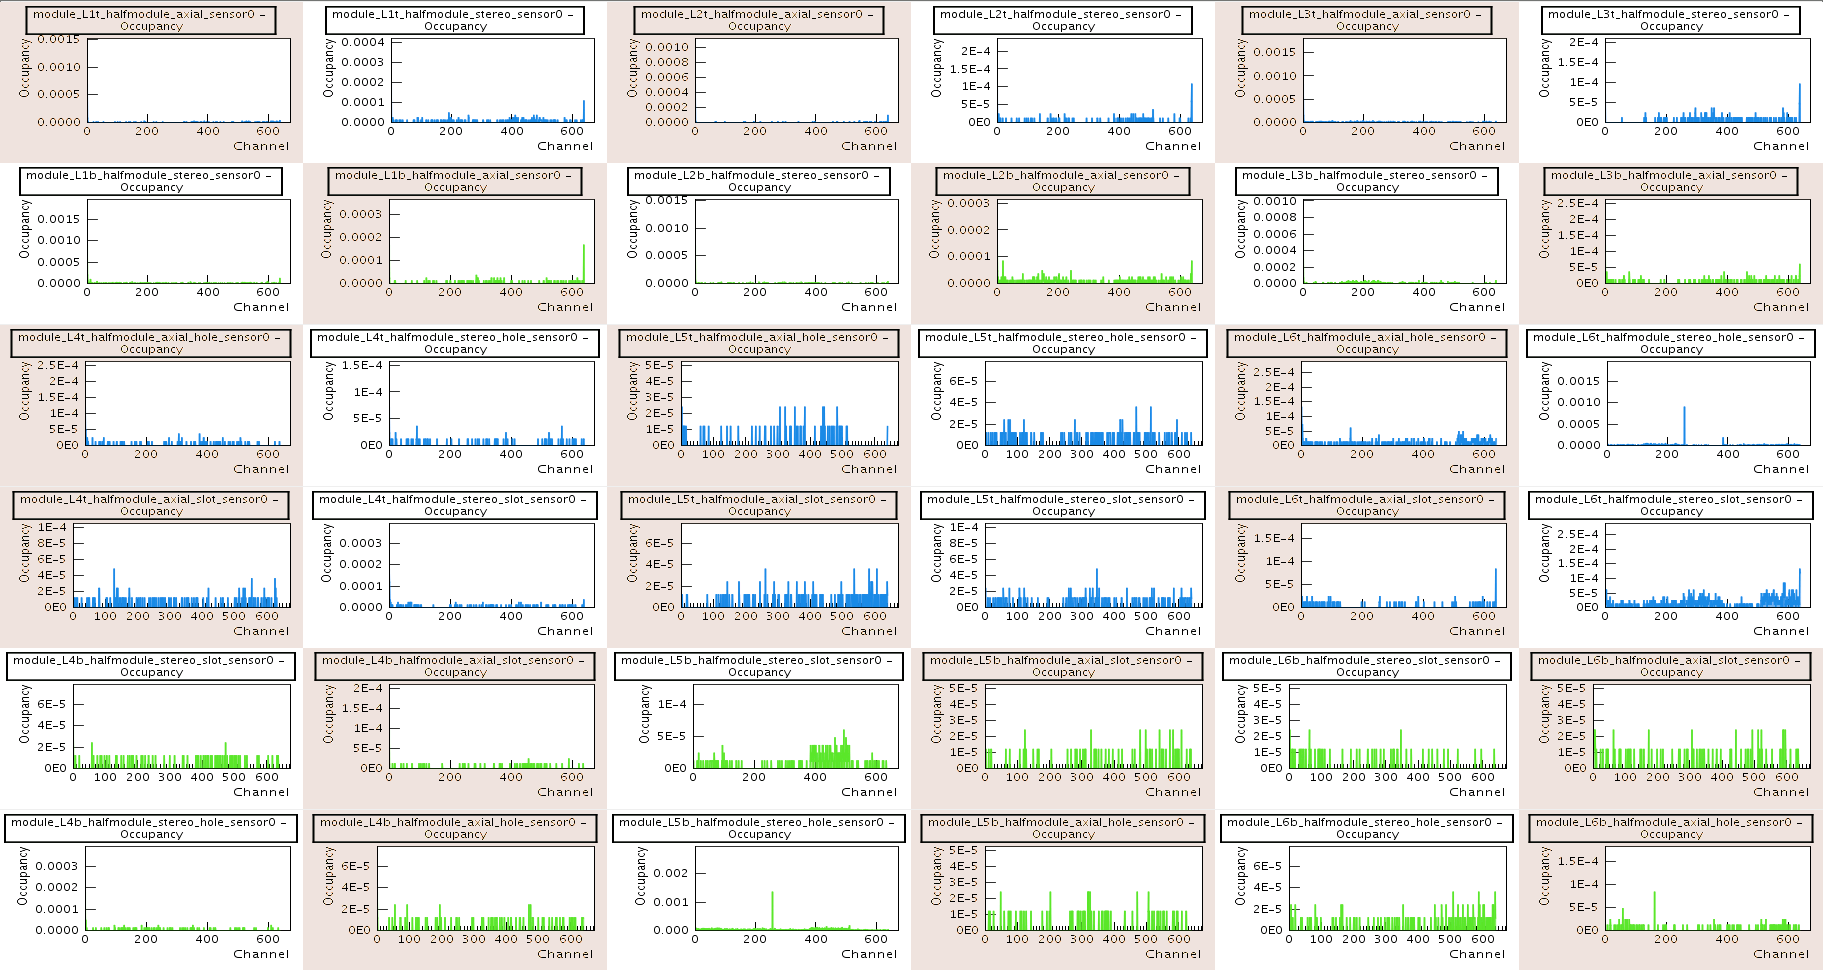
\includegraphics[width=\textwidth]{figures/occupancy_monitoring_app.png}
    \caption{SVT occupancies plot.}
    \label{fig:occupancies}
\end{figure}

\subsection {SVT Hits}

\subsection {Samples}


